

\chapter{Linked list}
\label{cha:linked-list}

Similar to the array, the linked list is also a linear data structure. Here is an example in Figure \ref{fig:singly-linked-list} and \ref{fig:doubly-linked-list}:



\begin{figure}[!ht]
  \centering

  \begin{tikzpicture}[list/.style={rectangle split, rectangle split parts=2,
    draw, rectangle split horizontal}, >=stealth, start chain]

  % create the four node
  \node[list,on chain] (A) {12};
  \node[list,on chain] (B) {99};
  \node[list,on chain] (C) {37};
  \node[on chain,draw,inner sep=6pt] (D) {};
  % draw the cross
  \draw (D.north east) -- (D.south west); 
  \draw (D.north west) -- (D.south east);
  
  \draw[*->] let \p1 = (A.two), \p2 = (A.center) in (\x1,\y2) -- (B);
  \draw[*->] let \p1 = (B.two), \p2 = (B.center) in (\x1,\y2) -- (C);
  \draw[*->] let \p1 = (C.two), \p2 = (C.center) in (\x1,\y2) -- (D);
\end{tikzpicture}

  \caption{Singly linked list}
  \label{fig:singly-linked-list}
\end{figure}

\begin{figure}[!ht]
  \centering
  \begin{tikzpicture}[list/.style={rectangle split, rectangle split parts=3,
    draw, rectangle split horizontal}, >=stealth, start chain]

  % create the four node
  \node[on chain,draw,inner sep=6pt] (E) {};
  \node[list,on chain] (A) {\nodepart{second} 12};
  \node[list,on chain] (B) {\nodepart{second} 99};
  \node[list,on chain] (C) {\nodepart{second} 37};
  \node[on chain,draw,inner sep=6pt] (D) {};

  % draw the cross
  \draw (D.north east) -- (D.south west); 
  \draw (D.north west) -- (D.south east);
  \draw (E.north east) -- (E.south west); 
  \draw (E.north west) -- (E.south east);
  
  \draw[*->] let \p1 = (A.three), \p2 = (A.center) in (\x1,\y2)  -- (B);
  \draw[*->] let \p1 = (B.three), \p2 = (B.center) in (\x1,\y2)  -- (C);
  \draw[*->] let \p1 = (C.three), \p2 = (C.center) in (\x1,\y2) -- (D);

  \draw[*->] let \p1 = ($(B.one)+(0.15,0)$), \p2 = (B.center) in (\x1,\y2)  -- (A);
  \draw[*->] let \p1 = ($(C.one)+(0.15,0)$), \p2 = (C.center) in (\x1,\y2)  -- (B);
  \draw[*->] let \p1 = ($(A.one)+(0.15,0)$), \p2 = (A.center) in (\x1,\y2) -- (E);



\end{tikzpicture}  

  \caption{Doubly linked list}
  \label{fig:doubly-linked-list}
\end{figure}


As you can see, each element in the linked list is actually a separate object while all the objects are linked together by the reference field in each element.



\section{Singly linked list}
\label{sec:singly-linked-list}

In a singly linked list, each node in a singly-linked list contains not only the value but also a reference field to link to the next node. 

\subsection{Insert}

Figure \ref{fig:insert-into-linked-list} shows the operations to add a new value after a given node \keyword{prev}.

\begin{figure}[!ht]
  \centering
  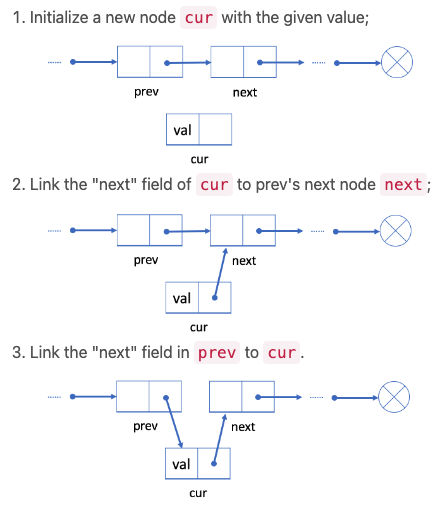
\includegraphics[width=0.6\textwidth]{/insert-into-singly-linked-list.png}
  \caption{Insert into singled linked list}
  \label{fig:insert-into-linked-list}
\end{figure}



\subsection{Delete}


Figure \ref{fig:delete-from-singled-linked-list} shows the operations to delete an existing node \keyword{cur} from the singly linked list.

\begin{figure}[!ht]
  \centering
  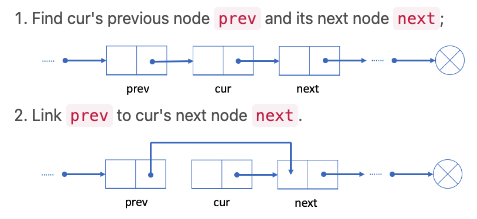
\includegraphics[width=0.6\textwidth]{/delete-from-singled-linked-list.png}
  \caption{Delete from singled linked list}
  \label{fig:delete-from-singled-linked-list}
\end{figure}



\section{Doubly Linked List}
\label{sec:doubly-linked-list}

The doubly linked list works in a similar way but has one more reference field which is known as the ``prev'' field.
With this extra field, you are able to know the previous node of the current node.


\subsection{Add Operation}
\label{sec:add-operation}

If we want to insert a new node \keyword{cur} after an existing node \keyword{prev}, we can divide this process into two steps as shown in Figure \ref{fig:add-to-doubly-linked-list}.
\begin{figure}[!ht]
  \centering
  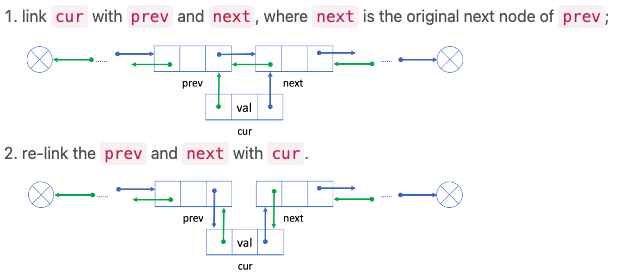
\includegraphics[width=0.8\textwidth]{/add-to-doubly-linked-list.png}
  \caption{Add to linked list}
  \label{fig:add-to-doubly-linked-list}
\end{figure}



\subsection{Delete Operation}
\label{sec:delete-operation}

If we want to delete an existing node \keyword{cur} from the doubly linked list, we can simply link its previous node \keyword{prev} with its next node \keyword{next}.



\section{Comparison}
\label{sec:comparison}



Here we provide a comparison of time complexity between the linked list and the array shown in Figure \ref{fig:array-and-linked-list}.
\begin{figure}[!ht]
  \centering
  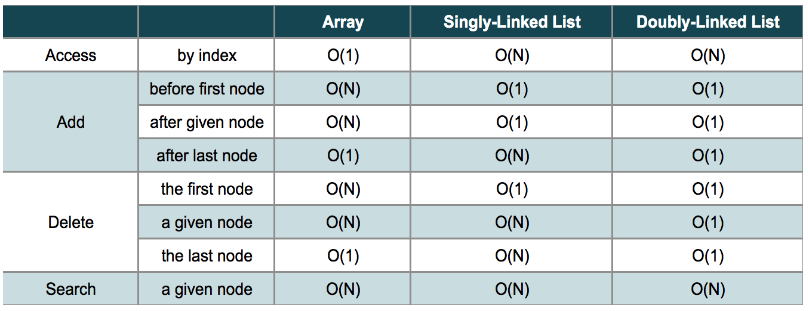
\includegraphics[width=0.8\textwidth]{/array-linked-list-comparison.png}
  \caption{Array and Linked List}
  \label{fig:array-and-linked-list}
\end{figure}


\section{Examples}
\label{sec:examples}


Here are some codes about linked list on \href{https://github.com/mingmingli916/algorithms/tree/main/linked_list}{Github}.



%%% Local Variables:
%%% mode: latex
%%% TeX-master: "algorithms"
%%% End:
